\subsection{UC-13 Modifica del profilo personale} 

\begin{figure}[H]
	\centering
	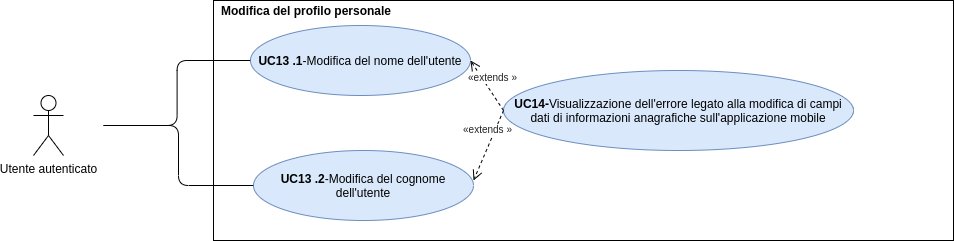
\includegraphics[width=\textwidth]{src/CasiDUso/immagini/SottocasiModificaProfilo.png}
	\caption{UC-13,14}
\end{figure}

\begin{itemize}

	\item \textbf{Attore primario:} utente autenticato;

	\item \textbf{Precondizioni:} l'utente è autenticato presso il sistema e si trova nella sezione "il mio profilo" dell'applicazione mobile;

	\item \textbf{Postcondizioni:} l'utente ha modificato uno o più campi relativi alle informazioni personali;

	\item \textbf{Scenario principale:} 
	
		\begin{enumerate}
    		\item  l'utente seleziona la funzionalità di modifica del profilo;
    		\item  l'utente seleziona il campo dati da modificare. L'utente può modificare:
    		
    			\begin{itemize}
        			\item il proprio nome (UC-12.1); 
        			\item il proprio cognome (UC-12.2); 
    			\end{itemize} 
    			
    		\item l'utente salva le modifiche apportate ai dati personali concludendo l'operazione di modifica.
    		
		\end{enumerate}
		
\end{itemize}


\subsubsection{UC-13.1 Modifica del nome dell'utente}

\begin{itemize}

	\item \textbf{Attore primario:} utente autenticato;

	\item \textbf{Precondizioni:} l'utente è autenticato presso il sistema e vuole modificare il proprio nome nella sezione "il mio profilo" dell'applicazione mobile;

	\item \textbf{Postcondizioni:} l'utente ha modificato il proprio nome della sezione "il mio profilo" dell'applicazione mobile;

	\item \textbf{Scenario principale:}
	
		\begin{enumerate}
   		 	\item l'utente seleziona la funzionalità di modifica del profilo;
   		 	\item l'utente seleziona il campo dati contenente il proprio nome;
   		 	\item l'utente salva le modifiche apportate al proprio nome concludendo l'operazione.
		\end{enumerate}
		
	\item \textbf{Estensioni:}
		\begin{enumerate}
    		\item UC-14 Visualizzazione dell'errore legato alla modifica di campi dati di informazioni anagrafiche sull'applicazione mobile.
		\end{enumerate}
		
\end{itemize}


\subsubsection{UC-13.2 Modifica del cognome dell'utente}
\begin{itemize}
	\item \textbf{Attore primario:} utente registrato;

	\item \textbf{Precondizioni:} l'utente è autenticato presso il sistema e vuole modificare il proprio cognome nella sezione "il mio profilo" dell'applicazione mobile;

	\item \textbf{Postcondizioni:} l'utente ha modificato il proprio cognome della sezione "il mio profilo" dell'applicazione mobile;

	\item \textbf{Scenario principale:}
	
		\begin{enumerate}
    		\item l'utente seleziona la funzionalità di modifica del profilo;
    		\item l'utente seleziona il campo dati contenente il proprio cognome;
    		\item l'utente salva le modifiche apportate al proprio nome concludendo l'operazione.
		\end{enumerate}
		
	\item \textbf{Estensioni:} 
	\begin{enumerate}
    	\item UC-14 Visualizzazione dell'errore legato alla modifica di campi dati di informazioni anagrafiche sull'applicazione mobile.
	\end{enumerate}
\end{itemize}


\subsection{UC-14 Visualizzazione dell'errore legato alla modifica di campi dati di informazioni anagrafiche sull'applicazione mobile}
\begin{itemize}
	\item \textbf{Attore primario:} utente autenticato;

	\item \textbf{Descrizione:} l'utente ha provato a modificare i propri dati anagrafici (nome,cognome) da applicazione mobile ma ha inserito delle stringhe non valide (es.contengono numeri o caratteri speciali).Viene pertanto visualizzato un errore esplicativo e le modifiche non vengono apportate;

	\item \textbf{Precondizioni:} l'utente ha provato a modificare i propri dati anagrafici (nome,cognome) da applicazione mobile ma ha inserito delle stringhe non valide (es.contengono numeri o caratteri speciali) e ha salvato le modifiche;

	\item \textbf{Postcondizioni:} il sistema restituisce un messaggio d'errore esplicativo e non completa la modifica dei dati anagrafici;

	\item \textbf{Scenario principale:}
	
		\begin{enumerate}
   			 \item il sistema elabora la richiesta ricevuta;
    		 \item il sistema restituisce un messaggio d'errore esplicativo che viene visualizzato sullo schermo del dispositivo dell'utente e non completa la modifica dei dati anagrafici.
		\end{enumerate}
\end{itemize}

\subsection{UC-15 Cancellazione del profilo di un impiegato da parte dell'amministratore}
\begin{itemize}
	\item \textbf{Attore primario:} amministratore autenticato;

	\item \textbf{Descrizione:} l'amministratore vuole cancellare un qualsiasi profilo di un impiegato;

	\item \textbf{Precondizioni:} l'amministratore è autenticato presso il sistema e accede alla schermata riepilogativa degli impiegati registrati;

	\item \textbf{Postcondizioni:} l'amministratore ha cancellato con successo il profilo di un impiegato registrato nel sistema;

	\item \textbf{Scenario principale:}
	
	\begin{enumerate}
    	\item l'amministratore seleziona la funzionalità di cancellazione di un impiegato registrato;
   	    \item l'amministratore seleziona l'impiegato registrato da rimuovere dal sistema;
 	    \item il sistema elabora correttamente la richiesta di rimozione e rimuove il profilo dell'impiegato.
	\end{enumerate}

\end{itemize}


